%\chapter{Challenge 1: Lane following}
%\chaptermark{Lane following}
%\label{ch:LaneFollowing}

\section{Anforderungen und Herausforderungen}
\sectionmark{Anf} % short form for headlines on pages
% Gedankengang beschreiben
% Wie sind wir zur Lösung gekommen?
% Herausforderungen und Probleme nennen

\section{Ablaufdiagramm}
\sectionmark{Impl} % short form for headlines on pages
% Ablaufdiagramm und Beschreibung der Node

\begin{figure}[H]
    \centering
    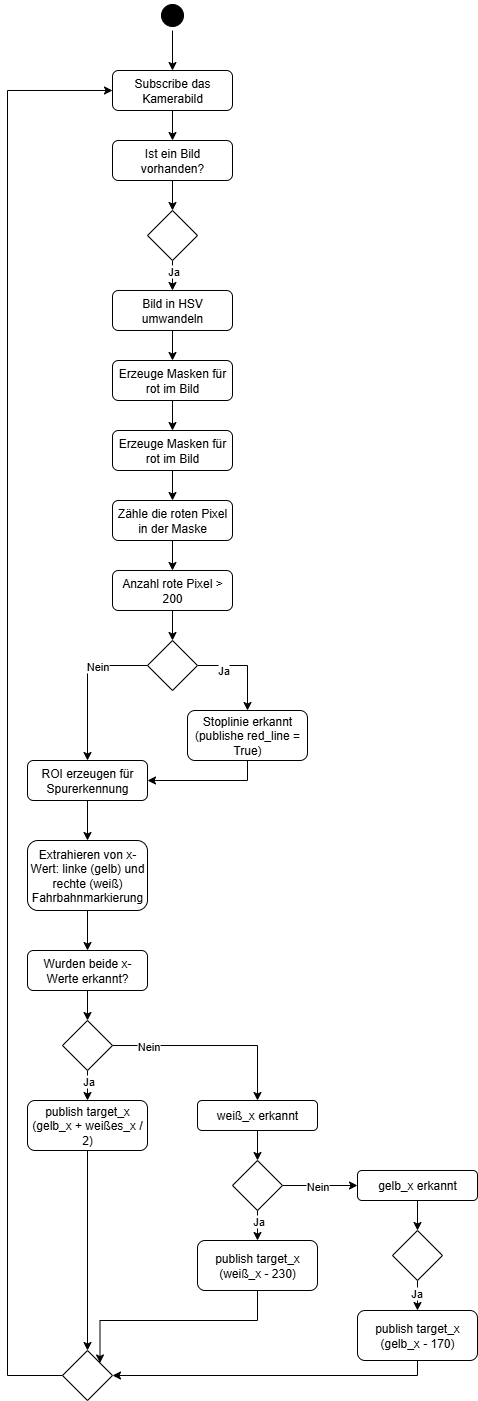
\includegraphics[width=0.8\textwidth]{Figures/png/Ablaufdiagramme_Bericht-Camera_reader.drawio.png}
    \caption{Ablaufdiagramm der Camera Reader Node}
    \label{fig:camera_reader_node}
\end{figure}

Die Camera-Reader-Node ist dafür verantwortlich, die Bilder der Frontkamera des Duckiebots zu empfangen und für die weitere Verarbeitung aufzubereiten. In Abbildung \ref{fig:camera_reader_node} ist das Ablaufdiagramm der Camera-Reader-Node dargestellt. Die Node beginnt mit der Initialisierung der Kamera und der ROS-Kommunikation. Anschließend wird in einer Endlosschleife kontinuierlich ein Bild von der Kamera empfangen. Dieses Bild wird dann in ein HSV-Bild umgewandelt. Dann wird das Bild auf die relevanten Farben rot, gelb und weiß gefiltert, um die Fahrbahnmarkierungen sowie die Stopp-Linien an Kreuzungen zu erkennen. Die x-Werte der erkannten Linien werden dann gepublished, um von anderen Nodes verarbeitet zu werden. Diese Informationen sind für die Spurverfolgung und die Navigation des Duckiebots essenziell.

\section{Technische Umsetzung im Code}
\sectionmark{Tech} % short form for headlines on pages
% Beschreibung wie man es im Code umgesetzt hat
Am Anfang der Node werden die Publisher und Subscriber initialisiert, um die Kommunikation mit anderen Nodes zu ermöglichen. In der run-Funktion wird das Bild in ein HSV-Bild umgewandelt und für weiß, gelb und rot eine Maske erstellt, mit denen im Bild nach den Farben gefiltert wird. Für die Erkennung einer roten Linie werden die erkannten roten Pixel gezählt und erst ab dem überschreiten des Schwellenwertes von 200 Pixeln wird die Linie als Linie erkannt. So kann gewährleistet werden, dass der Duckiebot nur auf eine Stopplinie reagiert und nicht auf andere rote Objekte, die im Bild auftauchen könnten.

Für die Erkennung der Fahrbahnmarkierungen der gelben Mittellinie und der weißen Seitenlinie wird mit Hilfe eines Canny-Filters die Kanten der Linien erkannt. Die am weitesten linke und rechte Kante wird dann aus allen Kanten extrahiert und gepublished. 









%% End of File %%